\documentclass[]{article}
\usepackage{lmodern}
\usepackage{amssymb,amsmath}
\usepackage{ifxetex,ifluatex}
\usepackage{fixltx2e} % provides \textsubscript
\ifnum 0\ifxetex 1\fi\ifluatex 1\fi=0 % if pdftex
  \usepackage[T1]{fontenc}
  \usepackage[utf8]{inputenc}
\else % if luatex or xelatex
  \ifxetex
    \usepackage{mathspec}
  \else
    \usepackage{fontspec}
  \fi
  \defaultfontfeatures{Ligatures=TeX,Scale=MatchLowercase}
\fi
% use upquote if available, for straight quotes in verbatim environments
\IfFileExists{upquote.sty}{\usepackage{upquote}}{}
% use microtype if available
\IfFileExists{microtype.sty}{%
\usepackage[]{microtype}
\UseMicrotypeSet[protrusion]{basicmath} % disable protrusion for tt fonts
}{}
\PassOptionsToPackage{hyphens}{url} % url is loaded by hyperref
\usepackage[unicode=true]{hyperref}
\hypersetup{
            pdftitle={slapnap: Super LeArner Prediction of NAb Panels},
            pdfauthor={David Benkeser, Brian D. Williamson, Craig A. Magaret, Bhavesh R. Borate, Peter B. Gilbert},
            pdfborder={0 0 0},
            breaklinks=true}
\urlstyle{same}  % don't use monospace font for urls
\usepackage[margin=1in]{geometry}
\usepackage{natbib}
\bibliographystyle{plainnat}
\usepackage{color}
\usepackage{fancyvrb}
\newcommand{\VerbBar}{|}
\newcommand{\VERB}{\Verb[commandchars=\\\{\}]}
\DefineVerbatimEnvironment{Highlighting}{Verbatim}{commandchars=\\\{\}}
% Add ',fontsize=\small' for more characters per line
\usepackage{framed}
\definecolor{shadecolor}{RGB}{248,248,248}
\newenvironment{Shaded}{\begin{snugshade}}{\end{snugshade}}
\newcommand{\KeywordTok}[1]{\textcolor[rgb]{0.13,0.29,0.53}{\textbf{#1}}}
\newcommand{\DataTypeTok}[1]{\textcolor[rgb]{0.13,0.29,0.53}{#1}}
\newcommand{\DecValTok}[1]{\textcolor[rgb]{0.00,0.00,0.81}{#1}}
\newcommand{\BaseNTok}[1]{\textcolor[rgb]{0.00,0.00,0.81}{#1}}
\newcommand{\FloatTok}[1]{\textcolor[rgb]{0.00,0.00,0.81}{#1}}
\newcommand{\ConstantTok}[1]{\textcolor[rgb]{0.00,0.00,0.00}{#1}}
\newcommand{\CharTok}[1]{\textcolor[rgb]{0.31,0.60,0.02}{#1}}
\newcommand{\SpecialCharTok}[1]{\textcolor[rgb]{0.00,0.00,0.00}{#1}}
\newcommand{\StringTok}[1]{\textcolor[rgb]{0.31,0.60,0.02}{#1}}
\newcommand{\VerbatimStringTok}[1]{\textcolor[rgb]{0.31,0.60,0.02}{#1}}
\newcommand{\SpecialStringTok}[1]{\textcolor[rgb]{0.31,0.60,0.02}{#1}}
\newcommand{\ImportTok}[1]{#1}
\newcommand{\CommentTok}[1]{\textcolor[rgb]{0.56,0.35,0.01}{\textit{#1}}}
\newcommand{\DocumentationTok}[1]{\textcolor[rgb]{0.56,0.35,0.01}{\textbf{\textit{#1}}}}
\newcommand{\AnnotationTok}[1]{\textcolor[rgb]{0.56,0.35,0.01}{\textbf{\textit{#1}}}}
\newcommand{\CommentVarTok}[1]{\textcolor[rgb]{0.56,0.35,0.01}{\textbf{\textit{#1}}}}
\newcommand{\OtherTok}[1]{\textcolor[rgb]{0.56,0.35,0.01}{#1}}
\newcommand{\FunctionTok}[1]{\textcolor[rgb]{0.00,0.00,0.00}{#1}}
\newcommand{\VariableTok}[1]{\textcolor[rgb]{0.00,0.00,0.00}{#1}}
\newcommand{\ControlFlowTok}[1]{\textcolor[rgb]{0.13,0.29,0.53}{\textbf{#1}}}
\newcommand{\OperatorTok}[1]{\textcolor[rgb]{0.81,0.36,0.00}{\textbf{#1}}}
\newcommand{\BuiltInTok}[1]{#1}
\newcommand{\ExtensionTok}[1]{#1}
\newcommand{\PreprocessorTok}[1]{\textcolor[rgb]{0.56,0.35,0.01}{\textit{#1}}}
\newcommand{\AttributeTok}[1]{\textcolor[rgb]{0.77,0.63,0.00}{#1}}
\newcommand{\RegionMarkerTok}[1]{#1}
\newcommand{\InformationTok}[1]{\textcolor[rgb]{0.56,0.35,0.01}{\textbf{\textit{#1}}}}
\newcommand{\WarningTok}[1]{\textcolor[rgb]{0.56,0.35,0.01}{\textbf{\textit{#1}}}}
\newcommand{\AlertTok}[1]{\textcolor[rgb]{0.94,0.16,0.16}{#1}}
\newcommand{\ErrorTok}[1]{\textcolor[rgb]{0.64,0.00,0.00}{\textbf{#1}}}
\newcommand{\NormalTok}[1]{#1}
\usepackage{longtable,booktabs}
% Fix footnotes in tables (requires footnote package)
\IfFileExists{footnote.sty}{\usepackage{footnote}\makesavenoteenv{long table}}{}
\usepackage{graphicx,grffile}
\makeatletter
\def\maxwidth{\ifdim\Gin@nat@width>\linewidth\linewidth\else\Gin@nat@width\fi}
\def\maxheight{\ifdim\Gin@nat@height>\textheight\textheight\else\Gin@nat@height\fi}
\makeatother
% Scale images if necessary, so that they will not overflow the page
% margins by default, and it is still possible to overwrite the defaults
% using explicit options in \includegraphics[width, height, ...]{}
\setkeys{Gin}{width=\maxwidth,height=\maxheight,keepaspectratio}
\IfFileExists{parskip.sty}{%
\usepackage{parskip}
}{% else
\setlength{\parindent}{0pt}
\setlength{\parskip}{6pt plus 2pt minus 1pt}
}
\setlength{\emergencystretch}{3em}  % prevent overfull lines
\providecommand{\tightlist}{%
  \setlength{\itemsep}{0pt}\setlength{\parskip}{0pt}}
\setcounter{secnumdepth}{5}
% Redefines (sub)paragraphs to behave more like sections
\ifx\paragraph\undefined\else
\let\oldparagraph\paragraph
\renewcommand{\paragraph}[1]{\oldparagraph{#1}\mbox{}}
\fi
\ifx\subparagraph\undefined\else
\let\oldsubparagraph\subparagraph
\renewcommand{\subparagraph}[1]{\oldsubparagraph{#1}\mbox{}}
\fi

% set default figure placement to htbp
\makeatletter
\def\fps@figure{htbp}
\makeatother


\title{\texttt{slapnap}: Super LeArner Prediction of NAb Panels}
\author{David Benkeser, Brian D. Williamson, Craig A. Magaret, Bhavesh R.
Borate, Peter B. Gilbert}
\date{May 28, 2020}

\begin{document}
\maketitle

{
\setcounter{tocdepth}{2}
\tableofcontents
}
\section*{Welcome}\label{welcome}
\addcontentsline{toc}{section}{Welcome}

The \href{https://hub.docker.com/r/slapnap/slapnap}{\texttt{slapnap}}
container is a tool for using the Compile, Analyze and Tally NAb Panels
(CATNAP) database to develop predictive models of HIV-1 neutralization
sensitivity to one or several broadly neutralizing antibodies (bNAbs).

\begin{center}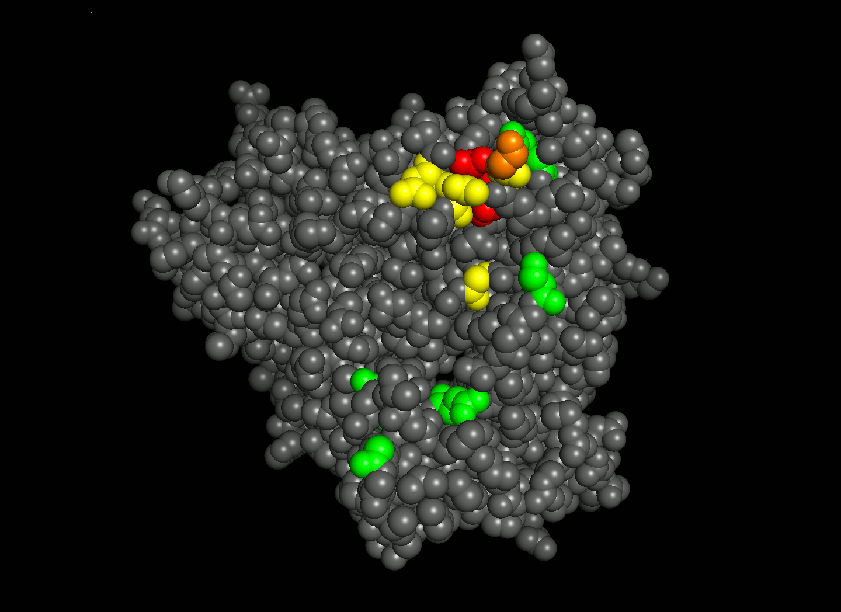
\includegraphics[width=0.7\linewidth]{gp120} \end{center}\begin{center}
Crystal structure of HIV-1 gp120 glycoprotein. Highlighted residues
indicating sites most-predictive of VRC01 neutralization resistance.
{[}@magaret2019prediction{]}
\end{center}

In its simplest form, \texttt{slapnap} can be used simply to access and
format data from CATNAP in a way that is usable for machine learning
analysis. However, the tool also offers fully automated and customizable
machine learning analyses based on up to five different neutralization
endpoints, complete with automated report generation to summarize
results and identify the most predictive features.

This document serves as the user manual for the \texttt{slapnap}
container. Here, we describe everything needed to utilize the
\texttt{slapnap} container and understand its output. The documentation
is organized into the following sections:

\begin{itemize}
\tightlist
\item
  Section \ref{sec:docker} provides a brief overview of Docker,
  including information on installing Docker and downloading the
  \texttt{slapnap} container.
\item
  Section \ref{sec:catnap} provides a brief overview of the CATNAP
  database and the specifics of how the data were accessed to build the
  \texttt{slapnap} container.
\item
  Section \ref{sec:runningcontainer} provides a detailed description of
  how to make calls to the slapnap repository, including descriptions of
  all options that are available.
\item
  Section \ref{sec:examples} includes several example calls to the
  \texttt{slapnap} container and descriptions of their output.
\item
  Section \ref{sec:data} provides a description of the data set created
  in the \texttt{slapnap} container.
\item
  Section \ref{sec:methods} provides an overview of the methodology that
  is used in within the \texttt{slapnap} analysis.
\end{itemize}

If you have any issues or questions about using \texttt{slapnap}, please
\href{https://github.com/benkeser/slapnap/issues}{file an issue} on
GitHub.

\section{Docker}\label{sec:docker}

Docker is a free platform for building containers. Containers are
standard units of software that package code and all its dependencies,
so that the code can be executed reliably irrespective of computing
environment. The \texttt{slapnap} tool relies on machine learning
implemented in the \texttt{R} language and relies on several packages.
Achieving full reproducibility for such analyses is challenging in that
it requires synchronization across the specific version of \texttt{R}
and dependent packages. In other words, two users running two versions
of \texttt{R} or two versions of the same \texttt{R} package may arrive
at different output when running the same code. Containerization ensures
that this does not happen. Any two runs of \texttt{slapnap} with the
same input options will yield the same output every time.

\href{https://docs.docker.com/docker-for-windows/install/}{Installing
Docker} is necessary for running the \texttt{slapnap} tool. While it is
not necessary for execution of the \texttt{slapnap} container, readers
interested in learning more about Docker should consult the
\href{https://docs.docker.com/get-started/}{Docker documentation} for
information about getting started using Docker.

Once Docker has been installed on your local computer, you can download
\texttt{slapnap} using the following command.

\begin{Shaded}
\begin{Highlighting}[]
\ExtensionTok{docker}\NormalTok{ pull slapnap/slapnap}
\end{Highlighting}
\end{Shaded}

This command pulls the image from
\href{https://hub.docker.com/}{DockerHub}. Once the image has been
downloaded, we are ready to learn about how to execute \texttt{slapnap}
jobs. The next section contains information on the source data used by
\texttt{slapnap}. Users familiar with the CATNAP data may wish to skip
directly to Section \ref{sec:opts}.

\section{CATNAP Database}\label{sec:catnap}

The
\href{https://www.hiv.lanl.gov/components/sequence/HIV/neutralization/index.html}{CATNAP
database} is a web server hosted by Los Alamos National Laboratory
\citep{yoon2015catnap}. The database integrates antibody neutralization
and HIV-1 sequence data from published studies. Neutralization is
measured in terms of half maximal inhibitory concentration (IC\(_{50}\))
and 80\% inhibitory concentration (IC\(_{80}\)). These measures of
neutralization against HIV envelope pseudoviruses are available for many
broadly neutralizing antibodies (bNAbs) and for some combination bNAbs.
Also available on each pseudovirus are amino acid (AA) sequence features
for the gp160 protein. These are detailed in Section \ref{sec:data}.

During each build of the \texttt{slapnap} container, all raw data are
downloaded from CATNAP. At run time, the relevant data are selected and
processed into a format that is amenable for predictive machine learning
analyses. The CATNAP data are updated periodically. To check the date
the raw data were pulled from CATNAP to \texttt{slapnap}, you can check
the date of the \texttt{latest} build
\href{https://hub.docker.com/repository/registry-1.docker.io/slapnap/slapnap/tags?page=1}{here}.

\section{\texorpdfstring{Running the \texttt{slapnap}
container}{Running the slapnap container}}\label{sec:runningcontainer}

To run the \texttt{slapnap} container, we make use of the
\href{https://docs.docker.com/engine/reference/run/}{\texttt{docker\ run}}
command. Note that administrator (\texttt{sudo}) privileges are needed
to execute this command.

There are several options that are necessary to include in this command
to control the behavior of \texttt{slapnap}. These are discussed in
separate subsections below.

\subsection{\texorpdfstring{\texttt{slapnap}
options}{slapnap options}}\label{sec:opts}

The user has control over many aspects of \texttt{slapnap}'s behavior.
These options are passed in using the \texttt{-e} option\footnote{This
  sets an environment variable in the container environment. These
  variables are accessed by the various \texttt{R} and \texttt{bash}
  scripts in the container to dictate how the container executes code.}.
Semi-colon separated strings are used to set options. For example, to
provide input for the option \texttt{option\_name}, we would used
\texttt{-e\ option\_name="a;semi-colon;separated;string"}. Note that
there are no spaces between the option name and its value and no spaces
after semi-colons in the separated list. See Section \ref{sec:examples}
for full syntax.

Each description below lists the default value that is assumed if the
option is not specified. Note that many of the default values are chosen
simply so that na\{"i\}ve calls to \texttt{slapnap} compile quickly.
Proper values should be determined based on scientific context.

\textbf{-e options for \texttt{slapnap}}

\begin{itemize}
\tightlist
\item
  \textbf{\texttt{nab}}: A semicolon-separated list of bNAbs (default =
  \texttt{"VRC01"}). A list of possible bNAbs can be found
  \href{https://www.hiv.lanl.gov/components/sequence/HIV/neutralization/main.comp}{here}.
  If multiple bNAbs are listed, it is assumed that the analysis should
  be of estimated \texttt{outcomes} for a combination of bNAbs (see
  Section \ref{sec:outcomedefs} for details on how estimated outcomes
  for multiple bNAbs are computed).
\item
  \textbf{\texttt{outcomes}}: A semicolon-separated string of outcomes
  to include in the analysis. Possible values are \texttt{"ic50"}
  (included in default), \texttt{"ic80"}, \texttt{"iip"},
  \texttt{"sens"} (included in default), \texttt{"estsens"},
  \texttt{"multsens"}. If only a single \texttt{nab} is specified, use
  \texttt{sens} to include a dichotomous endpoint. If multiple
  \texttt{nab}s are specified, use \texttt{estsens} and/or
  \texttt{multsens}. For detailed definitions of outcomes see Section
  \ref{sec:outcomedefs}).
\item
  \textbf{\texttt{sens\_thresh}} A numeric value defining the
  IC\(_{50}\) threshold for defining a sensitive versus resistant
  pseudovirus (default = 1). The dichotomous sensitivity/resistant
  \texttt{outcome}s are defined as the indicator that (estimated)
  IC\(_{50}\) is greater than or equal to \texttt{sens\_thresh}.
\item
  \textbf{\texttt{multsens\_nab}} A numeric value used for defining
  whether a pseudovirus is resistant to a multi-nAb cocktail. The
  dichotomous outcome \texttt{multsens} is defined as the indicator that
  a virus has (estimated) \(IC_{50}\) greater than \texttt{sens\_thresh}
  for at least \texttt{multsens\_nab} nAbs.
\item
  \textbf{\texttt{learners}}: A semicolon-separated string of machine
  learning algorithms to include in the analysis. Possible values
  include \texttt{"rf"} (random forest, default), \texttt{"xgboost"}
  (eXtreme gradient boosting), and \texttt{"lasso"} (elastic net). If
  more than one algorithm is included, then it is assumed that a
  cross-validated-based ensemble (i.e., a super learner) is desired (see
  Section \ref{sec:sldetails}).
\item
  \textbf{\texttt{cvtune}}: A boolean string (i.e., either
  \texttt{"TRUE"} or \texttt{"FALSE"} {[}default{]}) indicating whether
  the \texttt{learners} should be tuned using cross-validation and a
  small grid search. Defaults to \texttt{"FALSE"}. If multiple
  \texttt{learners} are specified, then the super learner ensemble
  includes three versions of each of the requested \texttt{learners}
  with different tuning parameters.
\item
  \textbf{\texttt{cvperf}}: A boolean string (i.e., either
  \texttt{"TRUE"} or \texttt{"FALSE"} {[}default{]}) indicating whether
  the \texttt{learners} performance should be evaluated using
  cross-validation. If \texttt{cvtune="TRUE"} or \texttt{learners}
  includes multiple algorithms, then nested cross-validation is used to
  evaluate the performance of the cross-validation-selected best value
  of tuning parameters for the specified algorithm or the super learner,
  respectively.
\item
  \textbf{\texttt{nfolds}}: A numeric string indicating the number of
  folds to use in cross-validation procedures (default = \texttt{"2"}).
\item
  \textbf{\texttt{importance\_grp}}: A semicolon-separated string
  indicating which group-level variable importance measures should be
  computed. Possible values are none \texttt{""} (default), marginal
  \texttt{"marg"}, conditional \texttt{"cond"}. See Section
  \ref{sec:biolimp} for details on these measures.
\item
  \textbf{\texttt{importance\_ind}}: A semicolon-separated string
  indicating which individual-level variable importance measures should
  be computed. Possible values are none \texttt{""} (default),
  learner-level \texttt{"pred"}, marginal \texttt{"marg"} and
  conditional \texttt{"cond"}. The latter two take significant
  computation time to compute.
\item
  \textbf{\texttt{same\_subset}} If \texttt{"FALSE"} (default) all data
  available for each outcome will be used in the analysis. If
  \texttt{"TRUE"}, the data will be subset to just those sequences that
  have measured IC\(_{50}\), IC\(_{80}\), and for which IIP can be
  computed (i.e., measured IC\(_{50}\) and IC\(_{80}\) values are
  different). Thus, if \texttt{"TRUE"} all outcomes will be fit on the
  \texttt{same\_subset} of the CATNAP data.
\item
  \textbf{\texttt{report\_name}}: A string indicating the desired name
  of the output report (default =
  \texttt{report\_{[}\_-separated\ list\ of\ nabs{]}\_{[}date{]}.html}).
\item
  \textbf{\texttt{return}}: A semicolon-separated string of the desired
  output. Possible values are \texttt{"report"} (default),
  \texttt{"learner"} for the trained algorithm, \texttt{"data"} for the
  analysis dataset, \texttt{"figures"} for all figures from the report,
  and \texttt{"vimp"} for variable importance objects.
\item
  \textbf{\texttt{view\_port}}: A boolean string indicating whether the
  compiled report should be made viewable on \texttt{localhost} (default
  \texttt{"FALSE"}). If \texttt{"TRUE"} then \texttt{-p} option should
  be used in the \texttt{docker\ run} command to identify the port. See
  example in Section \ref{sec:webbrowse} for details.
\end{itemize}

\subsection{Mounting a local directory}\label{sec:mounting}

At the end of a \texttt{slapnap} run, user-specified output will be
saved (see option \texttt{return} in Section \ref{sec:opts}). To
retrieve these files from inside the container, we can
\href{https://docs.docker.com/storage/bind-mounts/}{\emph{mount}} a
local directory to an output directory (\texttt{/home/output/}) in the
container using the \texttt{-v} option. That is, all files in the
mounted local directory will be visible to programs running inside the
container and any items saved to the output directory in the container
(file path in the container \texttt{/home/output/}) will be available in
the mounted directory.

Suppose \texttt{/path/to/local/dir} is the file path on a local computer
in which we wish to save the output files from a \texttt{slapnap} run. A
\texttt{docker\ run} of \texttt{slapnap} would include the option
\texttt{-v\ /path/to/local/dir:/home/output}. After a run completes, the
requested output should be viewable in \texttt{/path/to/local/dir}. See
Section \ref{sec:examples} for full syntax.

\subsection{Viewing report in web browser}\label{sec:viewreport}

An alternative option to mounting local directories for viewing and
downloading the report is to set the \texttt{view\_port} option to
\texttt{"TRUE"} and open a port to the container via the \texttt{-p}
option in the \texttt{docker\ run} statement. In this case, rather than
exiting upon completion of the analysis, the container will continuing
to run and broadcast the compiled report to \texttt{localhost} at the
specified port (see examples below). The report can be downloaded from
the web browser directly in this way.

\subsection{Interactive sessions}\label{interactive-sessions}

To simply enter the container and poke around, use an interactive
session by including \texttt{-it} and overriding the container's
entry-point.

\begin{Shaded}
\begin{Highlighting}[]
\ExtensionTok{docker}\NormalTok{ run -it slapnap/slapnap /bin/bash}
\end{Highlighting}
\end{Shaded}

This will enter you into the container in a bash terminal. This may be
useful for exploring the file structure, examining versions of
\texttt{R} packages that are included in the container, etc.

\section{Examples}\label{sec:examples}

\subsection{\texorpdfstring{Basic call to
\texttt{slapnap}}{Basic call to slapnap}}\label{basic-call-to-slapnap}

A call to \texttt{slapnap} with all default options can be run using the
following command.

\begin{Shaded}
\begin{Highlighting}[]
\ExtensionTok{docker}\NormalTok{ run -v /path/to/local/dir:/home/output slapnap/slapnap}
\end{Highlighting}
\end{Shaded}

Note that this call mounts the local directory
\texttt{path/to/local/dir} to receive output from the container (Section
\ref{sec:mounting}).

When this command is executed, messages will print to indicate the
progress of the container. The first message will report the name of the
log file, which will appear in \texttt{/path/to/local/dir}. The
container will then compile an analytic data set from the CATNAP
database for the default antibody (VRC01), train the default learner
(random forest \citep{breiman2001}) for the default outcomes
(\texttt{ic50} and \texttt{sens}), evaluate its performance using
two-fold (default for \texttt{nfolds}) cross-validation, and compile a
report detailing the results, and place the compiled report in
\texttt{path/to/local/dir}.

\subsection{Viewing results in a web browser
\{sec:webbrowse\}}\label{viewing-results-in-a-web-browser-secwebbrowse}

To have the results viewable in a web browser execute the following
command (note the use of \texttt{\textbackslash{}} to break the
\texttt{bash} command over multiple lines).

\begin{Shaded}
\begin{Highlighting}[]
\ExtensionTok{docker}\NormalTok{ run -v /path/to/local/dir:/home/output \textbackslash{}}
\NormalTok{           -e view_port=}\StringTok{"TRUE"}\NormalTok{ -p 80:80 \textbackslash{}}
\NormalTok{           slapnap/slapnap}
\end{Highlighting}
\end{Shaded}

This command opens port 80 on the container. Once the report has been
compiled, the container will not close down automatically. Instead it
will continue to run, broadcasting the report to port 80. Open a web
browser on your computer and navigate to \texttt{localhost:80} and you
should see the compiled report. Many web browsers should allow
downloading of the report (e.g., by right-clicking and selecting save
\texttt{Save\ As...}).

The container will continue to run until you tell it to \texttt{stop}.
To do that, retrieve the container ID by executing
\texttt{docker\ container\ ps}. Copy the ID of the running container
(say \texttt{MY\_CONTAINER\_ID}) and then execute
\texttt{docker\ stop\ MY\_CONTAINER\_ID} to shut down the container.

Note that in the above command, we have still mounted a local directory,
which may be considered best practice in case other output besides the
report is desired to be returned.

\subsection{Super learning}\label{super-learning}

If multiple \texttt{learner}s are specified, then a super learner
ensemble \citep{vanderlaan2007} is constructed. In the following
command, we construct an ensemble based on a random forest
\citep{breiman2001} and elastic net \citep{zou2005}. Note that the
execution time for super learners can be considerably greater than for
single \texttt{learner}s because of the extra layer of cross-validation
needed to construct the ensemble.

\begin{Shaded}
\begin{Highlighting}[]
\ExtensionTok{docker}\NormalTok{ run -v /path/to/local/dir:/home/output \textbackslash{}}
\NormalTok{           -e learners=}\StringTok{"rf;lasso"}\NormalTok{ \textbackslash{}}
\NormalTok{           slapnap/slapnap}
\end{Highlighting}
\end{Shaded}

\subsection{Train an algorithm}\label{train-an-algorithm}

The previous commands train learners and evaluate their performance
using cross-validation. However, at times we may wish only to use
\texttt{slapnap} to train a particular algorithm, while avoiding the
additional computational time associated with evaluating its
cross-validated performance and compiling a report. We show an example
of this below using sensitivity as the outcome.

\begin{Shaded}
\begin{Highlighting}[]
\ExtensionTok{docker}\NormalTok{ run -v /path/to/local/dir:/home/output \textbackslash{}}
\NormalTok{           -e learners=}\StringTok{"rf"}\NormalTok{ \textbackslash{}}
\NormalTok{           -e return=}\StringTok{"learner"}\NormalTok{ \textbackslash{}}
\NormalTok{           -e cvperf=}\StringTok{"FALSE"}\NormalTok{ \textbackslash{}}
\NormalTok{           -e outcome=}\StringTok{"sens"}\NormalTok{ \textbackslash{}}
\NormalTok{           slapnap/slapnap}
\end{Highlighting}
\end{Shaded}

After completion of this run, \texttt{learner\_sens.rds} will appear in
\texttt{/path/to/local/dir} that contains an \texttt{R} object of class
\texttt{ranger} (the package used by \texttt{slapnap} to fit random
forests).

\subsection{Pull and clean data}\label{pull-and-clean-data}

The \texttt{slapnap} container can also be used to return cleaned CATNAP
data suitable for analyses not supported by the \texttt{slapnap}
pipeline. In this case, the container avoids training machine learning
algorithms and report generation, returning a data set and associated
documentation. In the following call, \texttt{return} only includes
\texttt{"data"}; thus, options pertaining to the machine learning
portions of \texttt{slapnap} are essentially ignored by
\texttt{slapnap}. The inputted \texttt{outcomes} are also irrelevant, as
all \texttt{outcomes} are included in the resultant data set.

\begin{Shaded}
\begin{Highlighting}[]
\ExtensionTok{docker}\NormalTok{ run -v /path/to/local/dir:/home/output \textbackslash{}}
\NormalTok{           -e return=}\StringTok{"data"}\NormalTok{ \textbackslash{}}
\NormalTok{           slapnap/slapnap}
\end{Highlighting}
\end{Shaded}

\section{Report details}\label{sec:report}

\section{Data details}\label{sec:data}

\section{Method details}\label{sec:methods}

\subsection{Outcome definitions}\label{sec:outcomedefs}

\subsection{Super learner details}\label{sec:sldetails}

\subsection{Variable importance
details}\label{variable-importance-details}

If \texttt{importance\_grp} or \texttt{importance\_ind} is specified,
then variable importance estimates are computed based on the fitted
\texttt{learner}s. Both biological and prediction importance can be
obtained; we discuss each in the following two sections.

\subsubsection{Biological importance}\label{sec:biolimp}

Biological importance may be obtained by specifying
\texttt{importance\_grp}, \texttt{importance\_ind}, or both. We provide
two types of biological importance: marginal and conditional, accessed
by passing \texttt{"marg"} and \texttt{"cond"}, respectively, to one of
the importance variables. Both types of biological importance are based
on the population prediction potential of features
\citep{williamson2020}. We measure prediction potential using
nonparametric \(R^2\) for continuous outcomes (i.e., IC-50, IC-80, or
IIP) and using the nonparametric area under the receiver operating
characteristic curve (AUC) for binary outcomes (i.e., sensitivity,
estimated sensitivity, or multiple sensitivity). In both marginal and
conditional importance, we compare the population prediction potential
including the feature(s) of interest to the population prediction
potential excluding the feature(s) or interest; this provides a measure
of the biological importance of the feature(s). The two types of
biological importance differ only in the other adjustment variables that
we consider: conditional importance compares the prediction potential of
all features to the prediction potential of all features excluding the
feature(s) of interest, and thus importance must be interpreted
conditionally; whereas marginal importance compares the prediction
potential of the feature(s) of interest plus geographic confounders to
the prediction potential of the geographic confounders alone.

Both marginal and conditional biological importance can be computed for
groups of features or individual features. The available feature groups
are detailed in \ref{sec:data}. Execution time may increase dramatically
when biological importance is requested: a separate \texttt{learner} (or
super learner ensemble) must be trained for each feature group (or
individual feature) of interest. Marginal importance tends to be
computed more quickly than conditional importance, but both types of
importance provide useful information about the population of interest
and the underlying biology.

If feature importance is requested, then point estimates, confidence
intervals, and p-values (for a test of the null hypothesis that the
biological importance is equal to zero) will be computed and displayed
for each feature or group of features of interest.

In the following command, we request marginal biological importance for
the feature groups defined in \ref{sec:data}. We do not specify a super
learner ensemble to reduce computation time; however, in most problems
we recommend an ensemble to protect against model misspecification.

\begin{Shaded}
\begin{Highlighting}[]
\ExtensionTok{docker}\NormalTok{ run -v /path/to/local/dir:/home/output \textbackslash{}}
\NormalTok{           -e importance_grp=}\StringTok{"marg"}\NormalTok{ \textbackslash{}}
\NormalTok{           slapnap/slapnap}
\end{Highlighting}
\end{Shaded}

The raw \texttt{R} objects (saved as \texttt{.rds} files) containing the
point estimates, confidence intervals, and p-values for biological
importance can be saved by passing \texttt{"vimp"} to \texttt{return}.

\subsubsection{Predictive importance}\label{predictive-importance}

In addition to the biological importance, it may be of interest to
understand how the fitted \texttt{learner} depends on the measured
features. Learner-level predictive importance may be obtained by passing
\texttt{"pred"} to the variable \texttt{importance\_ind}. If a single
\texttt{learner} is fit, then the predictive importance is the
\texttt{R} default for that type of learner: for the elastic net,
importance is defined using the absolute value of the estimated
regression coefficient; for random forests, importance is defined using
the Gini index (binary outcomes) or the variance of the outcome
(continuous outcomes); for eXtreme gradient boosting \citep{chen2016},
importance is defined using the fractional contribution of total gain of
the feature's splits. If a super learner ensemble is fit, then the
best-fitting algorithm in the ensemble is used to compute the predictive
importance.

In the following command, we request predictive importance for a simple
scenario. Predictive importance is displayed for the top 20 features.

\begin{Shaded}
\begin{Highlighting}[]
\ExtensionTok{docker}\NormalTok{ run -v /path/to/local/dir:/home/output \textbackslash{}}
\NormalTok{           -e importance_ind=}\StringTok{"pred"}\NormalTok{ \textbackslash{}}
\NormalTok{           slapnap/slapnap}
\end{Highlighting}
\end{Shaded}

\section{References}\label{sec:refs}

\bibliography{refs.bib}

\end{document}
